\begin{figure}[h]
\centering
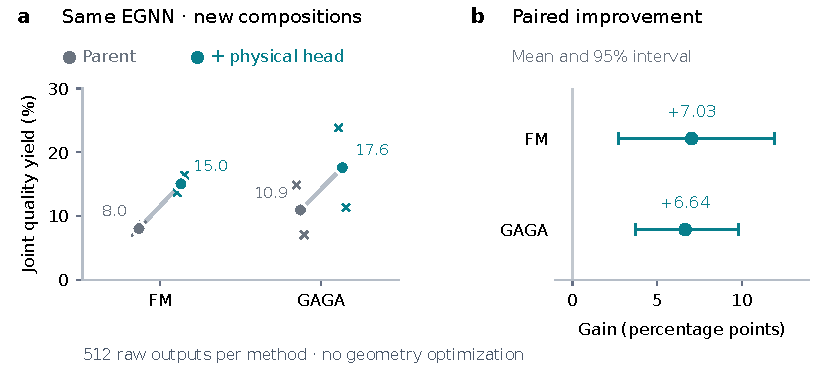
\includegraphics[width=\linewidth]{../research/figures/matched_connection_v1/matched_connection.pdf}
\caption{Physical correction transfers to independently trained EGNN generators.
(a) Joint yield requires an inferred valid graph and GFN2 force RMS at most
5 eV/\AA. Large circles show pooled rates; small crosses show the two fits.
(b) Within-parent improvements with paired composition-bootstrap 95\% intervals.
Both algorithms receive the same TRAIN compositions, force-query budget, head
architecture, and fitting schedule. All generated coordinates are unoptimized.}
\label{fig:matched-connection}
\end{figure}

\begin{table}[h]
\centering\small
\caption{Fresh shared-EGNN confirmation. Each row contains 512 attempts on the
same 16 compositions. The last two columns give joint yield in each independent
parent/head fit. Every GFN2 single-point calculation completed successfully.}
\begin{tabular}{lrrrr}
\toprule
Model & Graph (\%) & Joint (\%) & Fit 1 (\%) & Fit 2 (\%)\\
\midrule
FM, distance feedback &17.58&8.01&7.42&8.59\\
FM + physical head &20.31&15.04&13.67&16.41\\
GAGA &18.75&10.94&14.84&7.03\\
GAGA + physical head &20.31&17.58&23.83&11.33\\
\bottomrule
\end{tabular}\label{tab:matched-connection}
\end{table}

The primary FM comparison improves joint yield by 7.03 percentage points
(95\% interval $[2.73,11.91]$), with gains of 6.25 and 7.81 points in the two
fits. GAGA also benefits, gaining 6.64 points ($[3.71,9.77]$), with both fits
improving. Thus the learned correction transfers beyond the pretrained FlowMol
backbone and works with both velocity and noise prediction.

After identical physical supervision, FM minus GAGA is $-2.54$ points
($[-6.64,1.76]$). The difference between their within-parent improvements is
$+0.39$ points ($[-4.30,5.47]$). The experiment supports physical-head transfer
to both generators, while their ordering remains uncertain. Intervals resample
compositions and condition on the two fitted parents and heads; validation
strengths are fixed before test generation.
